\section{具体问题领域}

\subsection{情感分析结果需要二次展开}

\begin{spacing}{1.3}
    \centering
    \begin{longtable}{|W{c}{0.7cm}|m{5.5cm}|W{c}{2.5cm}|W{c}{2.5cm}|W{c}{2cm}|}
        \hline
        \textbf{No.} & \multicolumn{1}{c|}{\textbf{问题}}  & \textbf{严重程度排名} & \textbf{易于修复排名} & \textbf{启发式编号}\\ \hline
        1 & 情感分析结果需要二次展开 & 3 & 1 & 7,8 \\ \hline
    \end{longtable}
\end{spacing}

\subsubsection{问题}
在情感分析界面,注意到情感分析的打分和解释部分初始时是隐藏起来的,需要用户二次展开。这个问题违反了启发式7和8,这两个启发式建议设计起来应该使整个系统使用起来简单高效,为新手提供操作引导,同时要简洁美观,减少无关信息,取消没必要的操作。

\subsubsection{证据}
在情感分析界面,如图 \ref{问题1} 所示,“打分”和“解释”的具体内容为一个下拉菜单,需要下拉才能展开。

\begin{figure*}[t]
	\centering
	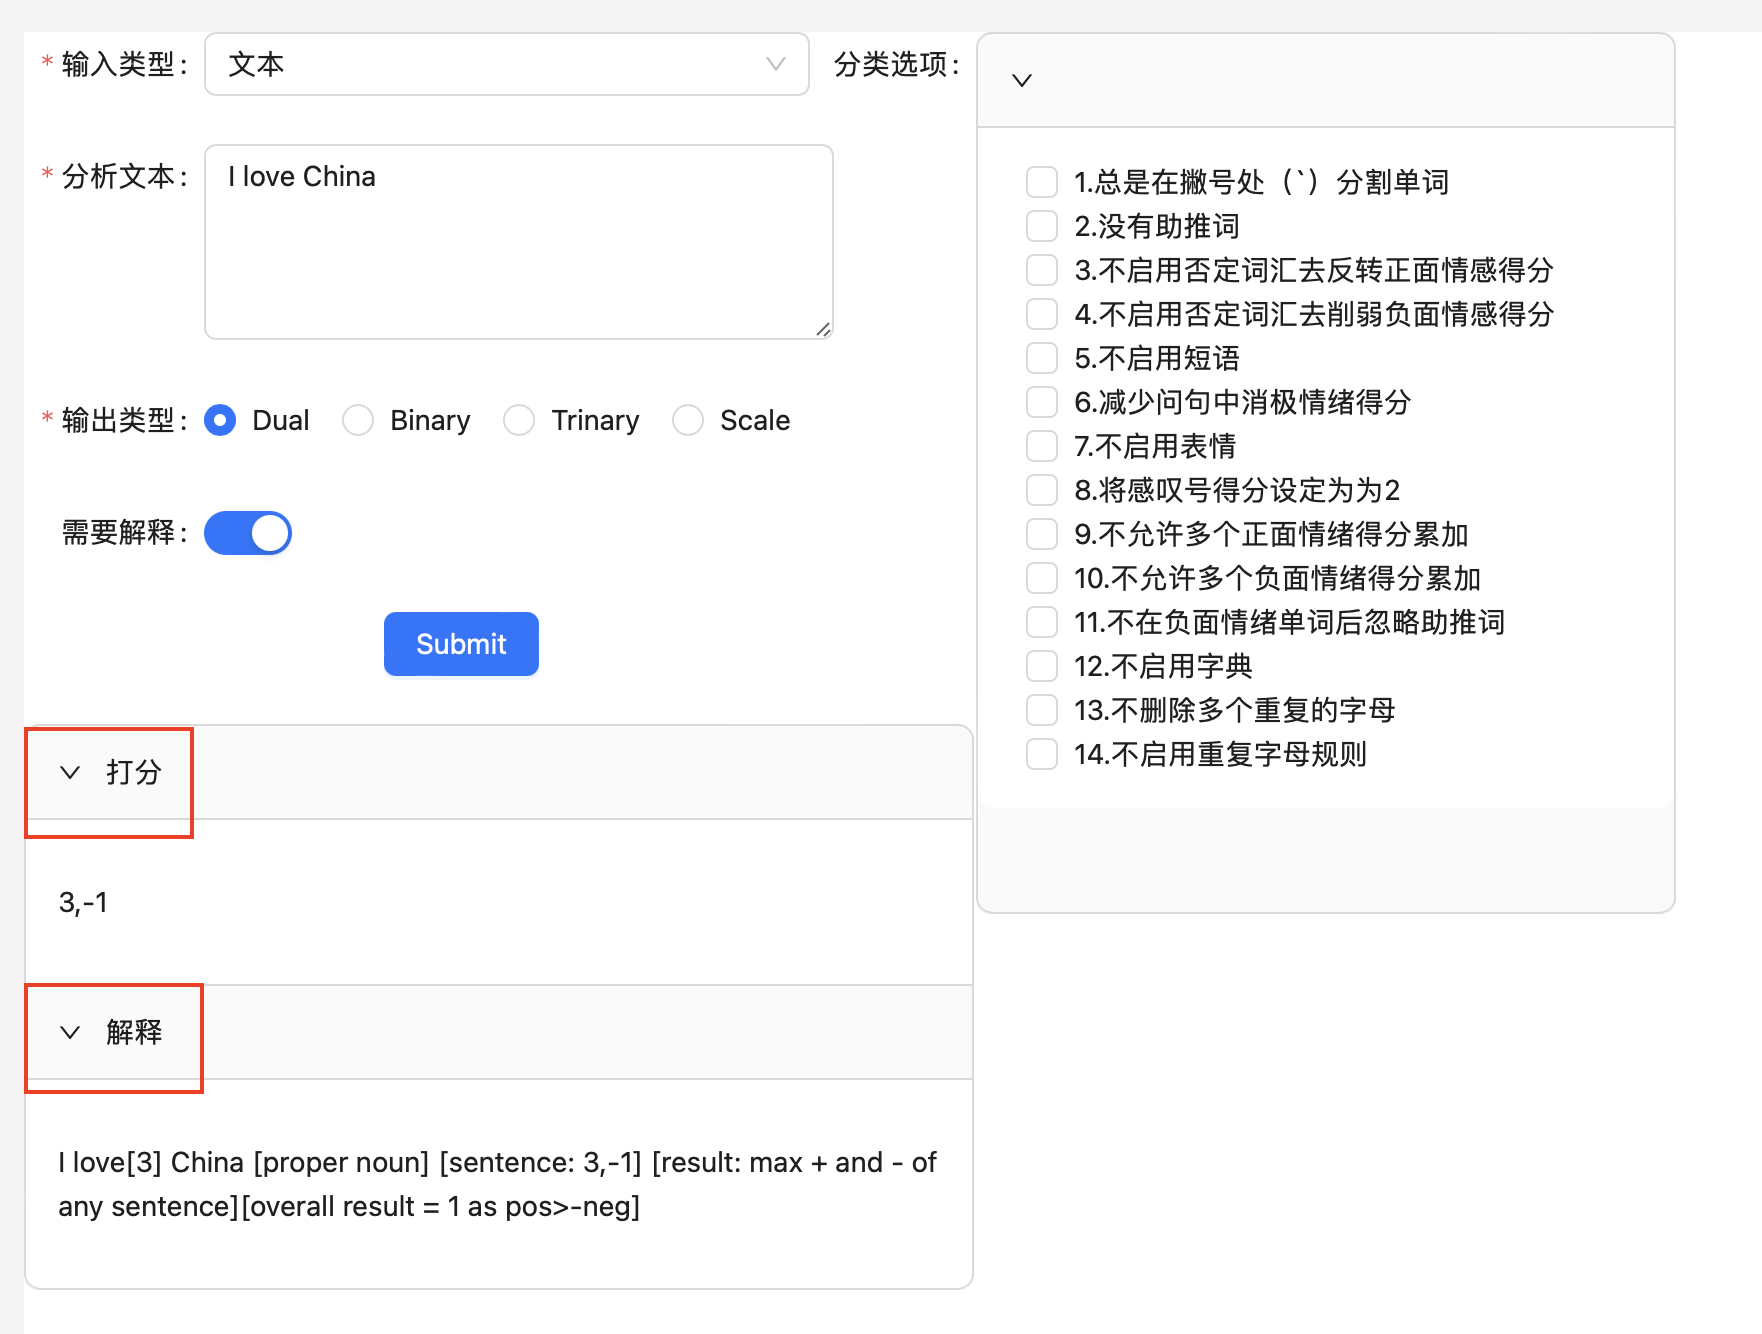
\includegraphics[width=0.98\textwidth]{images/问题1.png}
    \caption{情感分析结果需要二次展开}
    \label{问题1}
\end{figure*}

\subsubsection{建议}
解决这个问题并不难,仅涉及特定界面元素,解决方案明确,只需要设置打分和解释结果默认展开或者干脆取消下拉菜单即可。


\subsection{用户手册使用开发语言而不是用户语言}

\begin{spacing}{1.3}
    \centering
    \begin{longtable}{|W{c}{0.7cm}|m{5.5cm}|W{c}{2.5cm}|W{c}{2.5cm}|W{c}{2cm}|}
        \hline
        \textbf{No.} & \multicolumn{1}{c|}{\textbf{问题}}  & \textbf{严重程度排名} & \textbf{易于修复排名} & \textbf{启发式编号}\\ \hline
        2 & 用户手册使用开发语言而不是用户语言 & 3 & 1 & 2,7,10 \\ \hline
    \end{longtable}
\end{spacing}

\subsubsection{问题}
虽然该系统提供了用户手册,但所用语言过于偏向开发语言,而不是用户语言。这个问题违反了启发式2,7,10。这三个启发式建议系统使用用户语言,贴近实际生活,而不是使用学术概念;同时要对新手提供操作引导,对新手友好;最后提供人性化的帮助,用户帮助和文档要关注用户任务,列出具体的执行步骤,且不要太冗长。这个问题之所以列为可用性问题,是因为其不能通过用户的任何具体操作来解决。

\subsubsection{证据}
在用户手册界面,如图 \ref{问题2} 所示,虽然提供了用户手册,但所用语言对用户并不友好。

\begin{figure}[htbp]
	\centering
	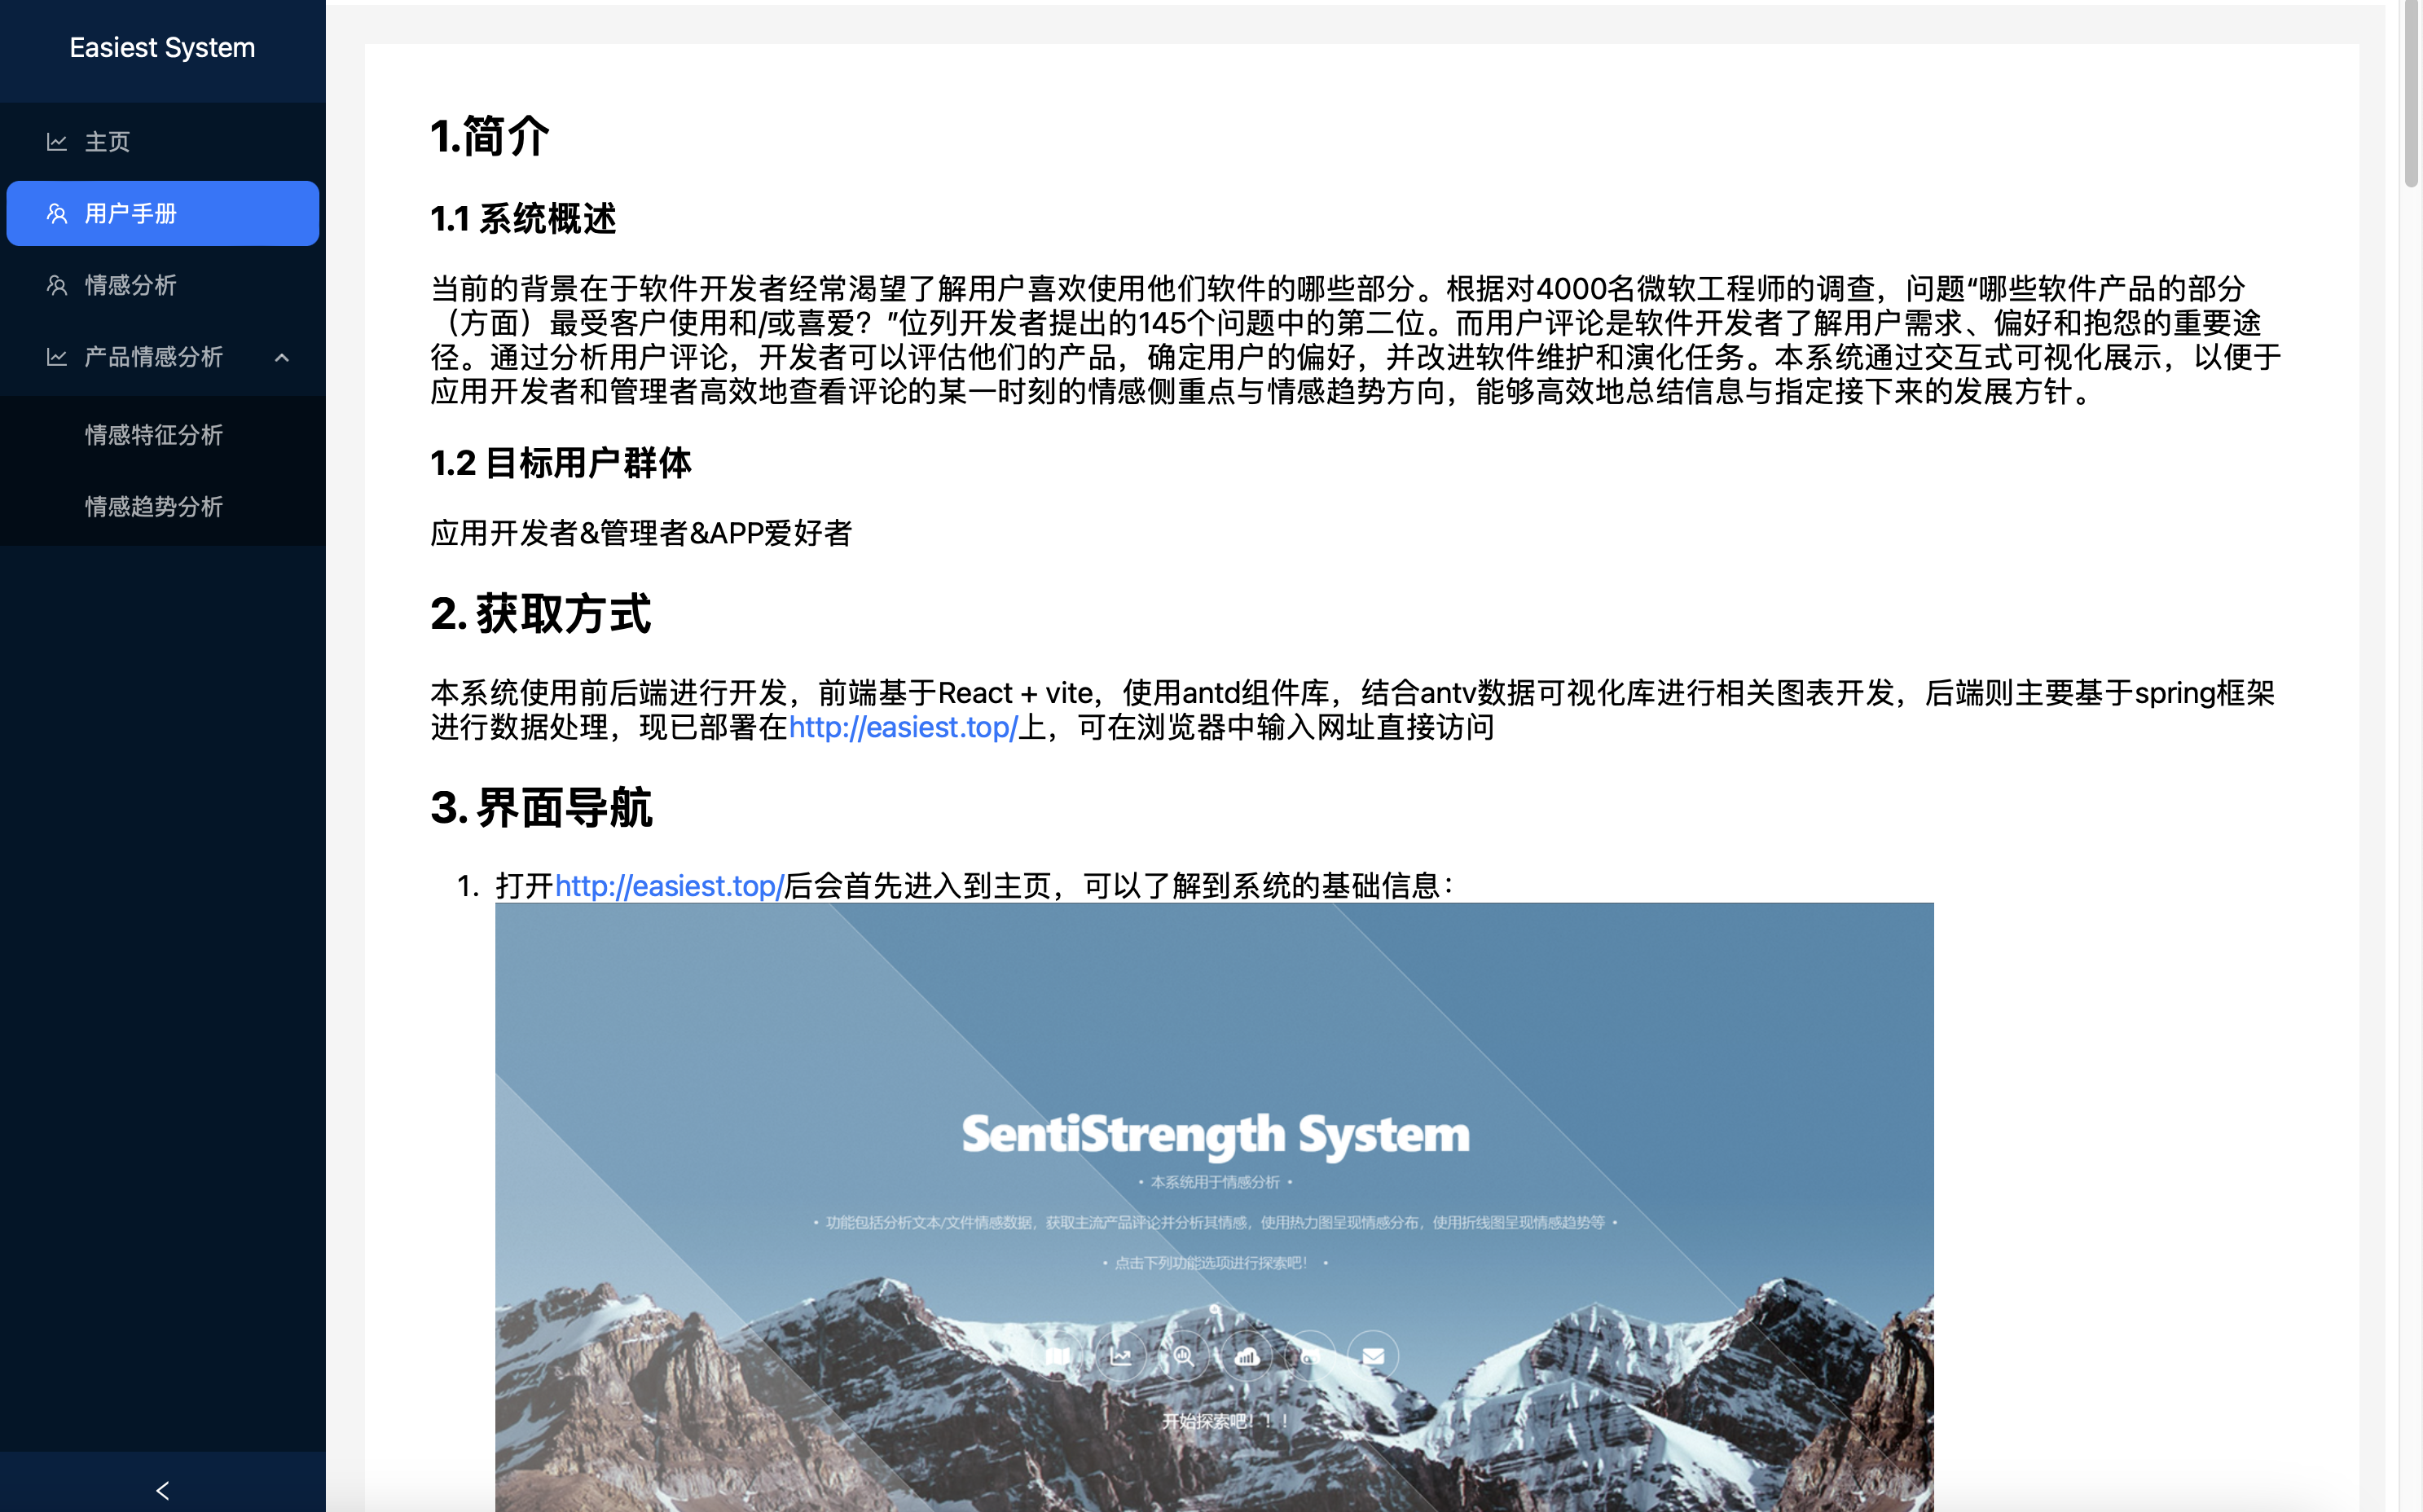
\includegraphics[width=0.98\textwidth]{images/问题2.png}
    \caption{用户手册使用开发语言而不是用户语言}
    \label{问题2}
\end{figure}

\subsubsection{建议}
要解决这个问题,最简单的方式就是对用户手册界面使用用户友好的语言进行重新编写。



\subsection{选择日期错误无法直接在选择界面更改}

\begin{spacing}{1.3}
    \centering
    \begin{longtable}{|W{c}{0.7cm}|m{5.5cm}|W{c}{2.5cm}|W{c}{2.5cm}|W{c}{2cm}|}
        \hline
        \textbf{No.} & \multicolumn{1}{c|}{\textbf{问题}}  & \textbf{严重程度排名} & \textbf{易于修复排名} & \textbf{启发式编号}\\ \hline
        3 & 选择日期错误无法直接在选择界面更改 & 2 & 2 & 3 \\ \hline
    \end{longtable}
\end{spacing}

\subsubsection{问题}
当选择日期错误时,无法直接在选择界面更改,而是需要将两个日期全部选完后,再重新点开日期选择框重新进行选择。这个问题违反了启发式3。这个启发式又称为撤销重做原则,即操作失误可退回:因为用户经常会误触系统功能,这时就需要一个清晰的“紧急出口”来离开非预期状态,而不是必须拓展一个新窗口。这个问题之所以列为可用性问题,是因为其不能通过用户的任何具体操作来解决。

\subsubsection{证据}
如图 \ref{问题3} 所示,当用户选择第一个日期后,前面的日期变得不可选,这种设计能够防止出现用户选择的后一个日期比前一个日期小的问题,但当用户第一个日期选择错误时,将难以进行更改,而是需要随机选择其后面一个日期将整个选择日期的行为完成后,再重新进行日期选择。

\begin{figure}[htp]
	\centering
	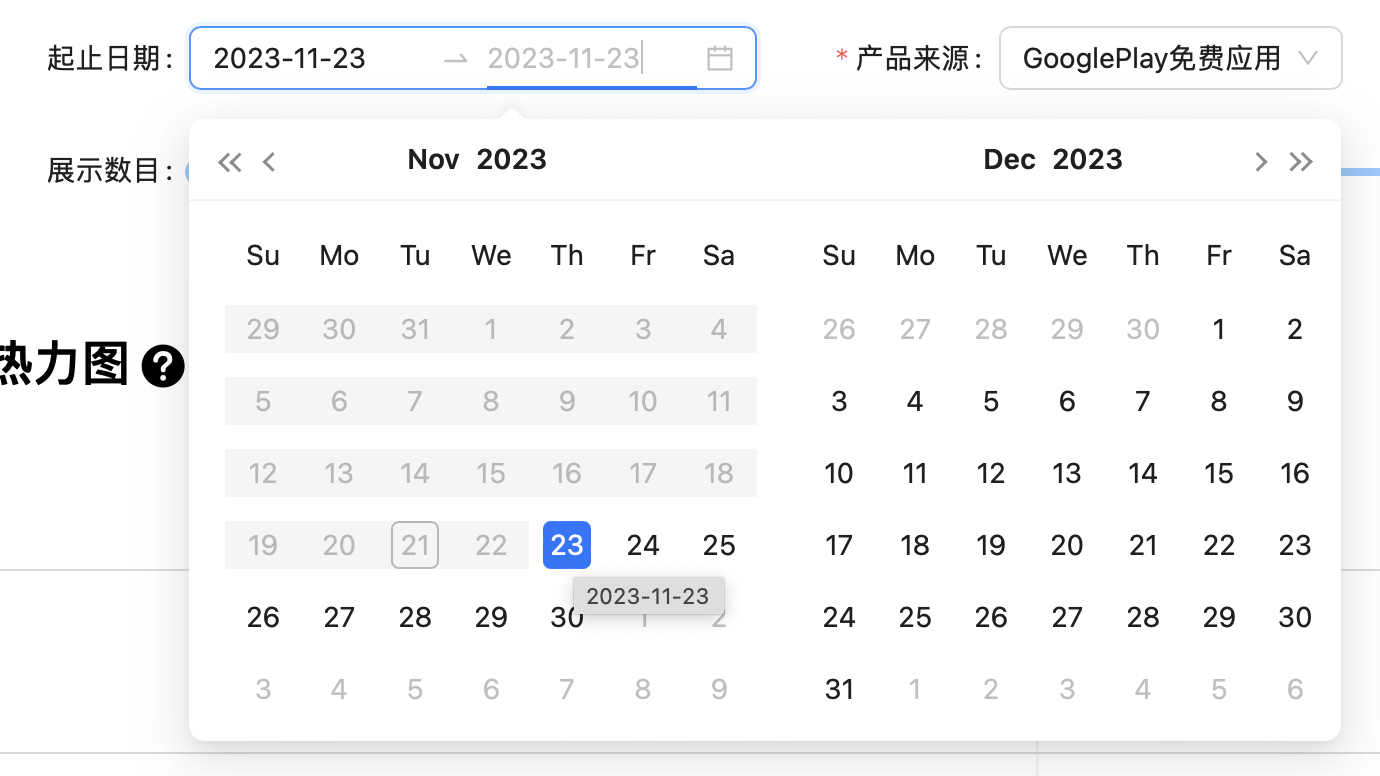
\includegraphics[width=0.7\textwidth]{images/问题3.png}
    \caption{选择日期错误无法直接在选择界面更改}
    \label{问题3}
\end{figure}

\subsubsection{建议}
解决这个问题需要修改日期选择的实现逻辑,当第一个日期已经选定后,不将用户选择这个日期前面的日期的行为视为错误的操作进行限制,而是认为用户是要进行修改,从而将第一个日期更新为所选择的前面日期。

\subsection{显示单词超出范围}

\begin{spacing}{1.3}
    \centering
    \begin{longtable}{|W{c}{0.7cm}|m{5.5cm}|W{c}{2.5cm}|W{c}{2.5cm}|W{c}{2cm}|}
        \hline
        \textbf{No.} & \multicolumn{1}{c|}{\textbf{问题}}  & \textbf{严重程度排名} & \textbf{易于修复排名} & \textbf{启发式编号}\\ \hline
        4 & 显示单词超出范围 & 2 & 3 & 4,8  \\ \hline
    \end{longtable}
\end{spacing}

\subsubsection{问题}
对于特征热力图的展示,原本的设计为每个圆圈表示自动提取的功能组,较大的圆圈表示更受欢迎和喜爱的功能,其中圆圈大小为$\log \mbox{评论数} + \mbox{情感得分}$。这样的设计从数学上看是直观的,但实际显示效果有很大问题。一是圆圈大小看上去都一样,没有什么区别;二是不同单词长度不一样,有的过长单词会显示在圆圈外面。这个问题违反了启发式4和8。

\subsubsection{证据}
如图 \ref{问题4} 所示,圆圈的大小几乎相同,同时过长的单词会超出圆圈的范围。

\begin{figure}[htp]
	\centering
	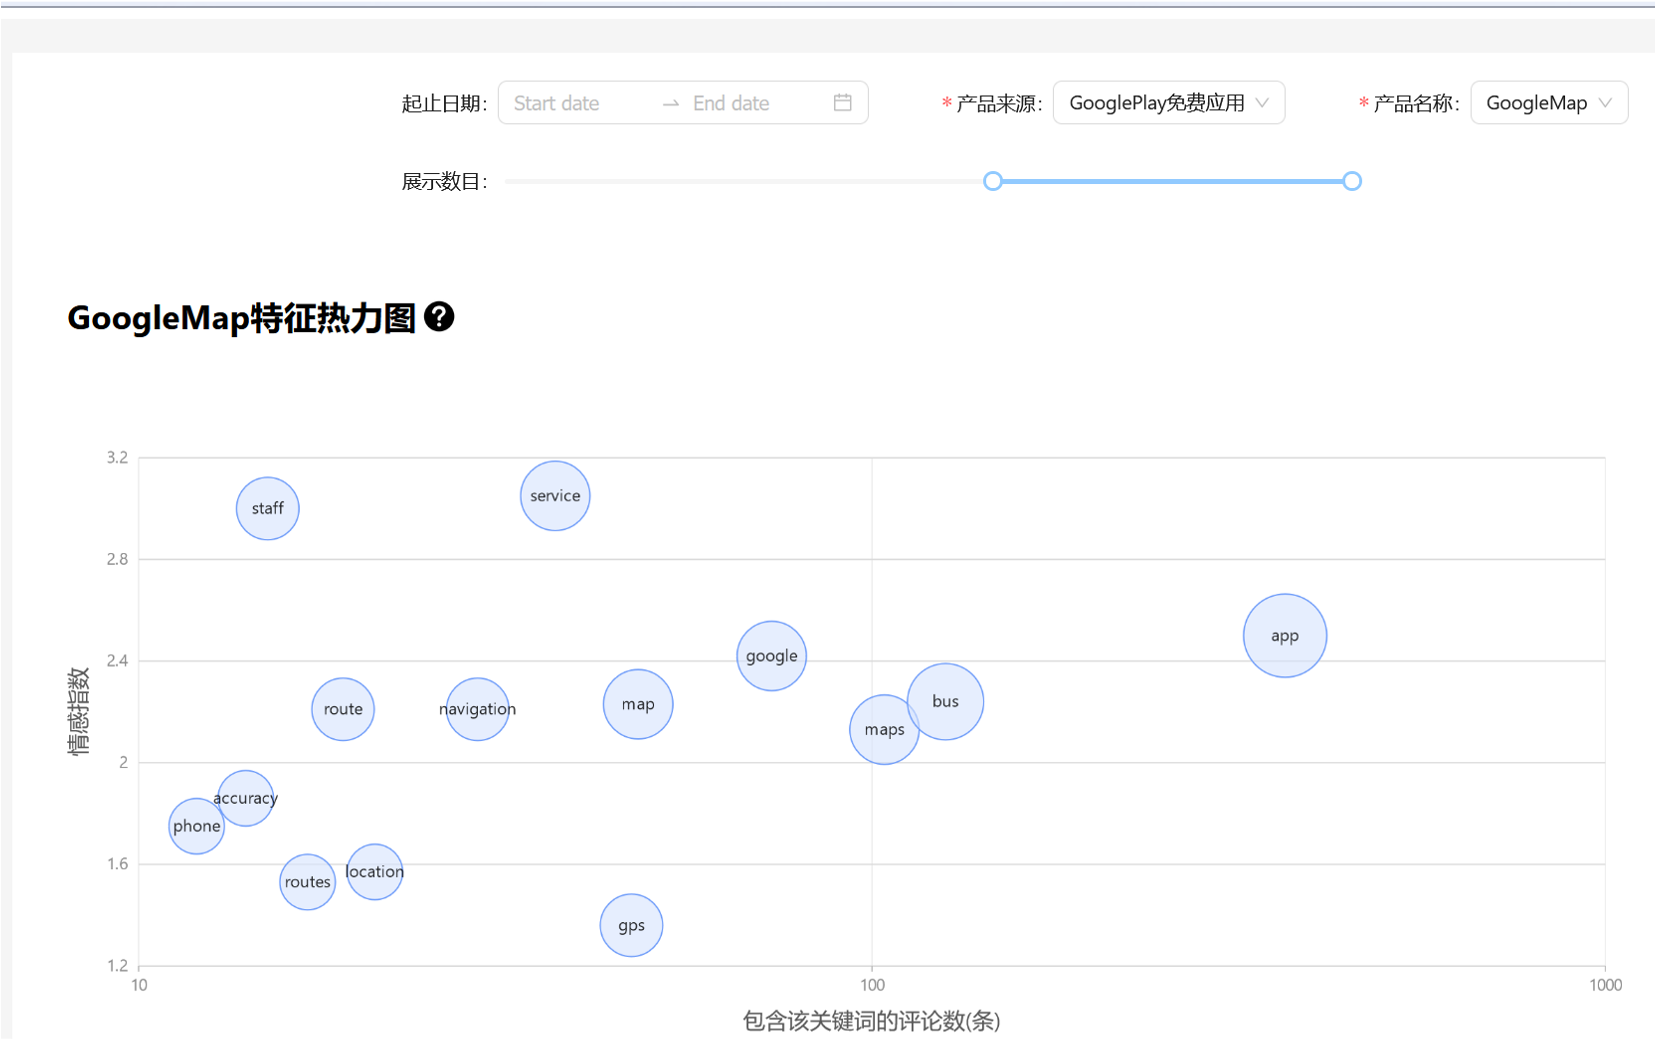
\includegraphics[width=0.98\textwidth]{images/问题4.png}
    \caption{显示单词超出范围}
    \label{问题4}
\end{figure}

\subsubsection{建议}
这个问题并不是很好解决,需要开发团队根据业务需求考虑重新设计圆圈大小的方式,同时根据单词长度进行动态调整字体大小等。


\subsection{页面使用无意义的初始值}

\begin{spacing}{1.3}
    \centering
    \begin{longtable}{|W{c}{0.7cm}|m{5.5cm}|W{c}{2.5cm}|W{c}{2.5cm}|W{c}{2cm}|}
        \hline
        \textbf{No.} & \multicolumn{1}{c|}{\textbf{问题}}  & \textbf{严重程度排名} & \textbf{易于修复排名} & \textbf{启发式编号}\\ \hline
        5 & 页面使用无意义的初始值 & 2 & 2 & 1,7 \\ \hline
    \end{longtable}
\end{spacing}

\subsubsection{问题}
在特征热力图和特征趋势图的初始界面中,也就是用户并没有选择APP和相关时间时,会显示一些无意义的初值,这违反了启发式1和7。无意义的初值的使用让用户并不知道系统在干什么,使系统状态不可见,为用户使用产生困扰。

\subsubsection{证据}
如图 \ref{问题5} 所示,两个界面的初始界面的显示值是无意义的。

\begin{figure}[htbp]
	\setcounter{subfigure}{0}
	\centering
	\subfloat[特征热力图初始界面]{
	    \begin{minipage}[t]{0.99\linewidth}
	    \centering
	    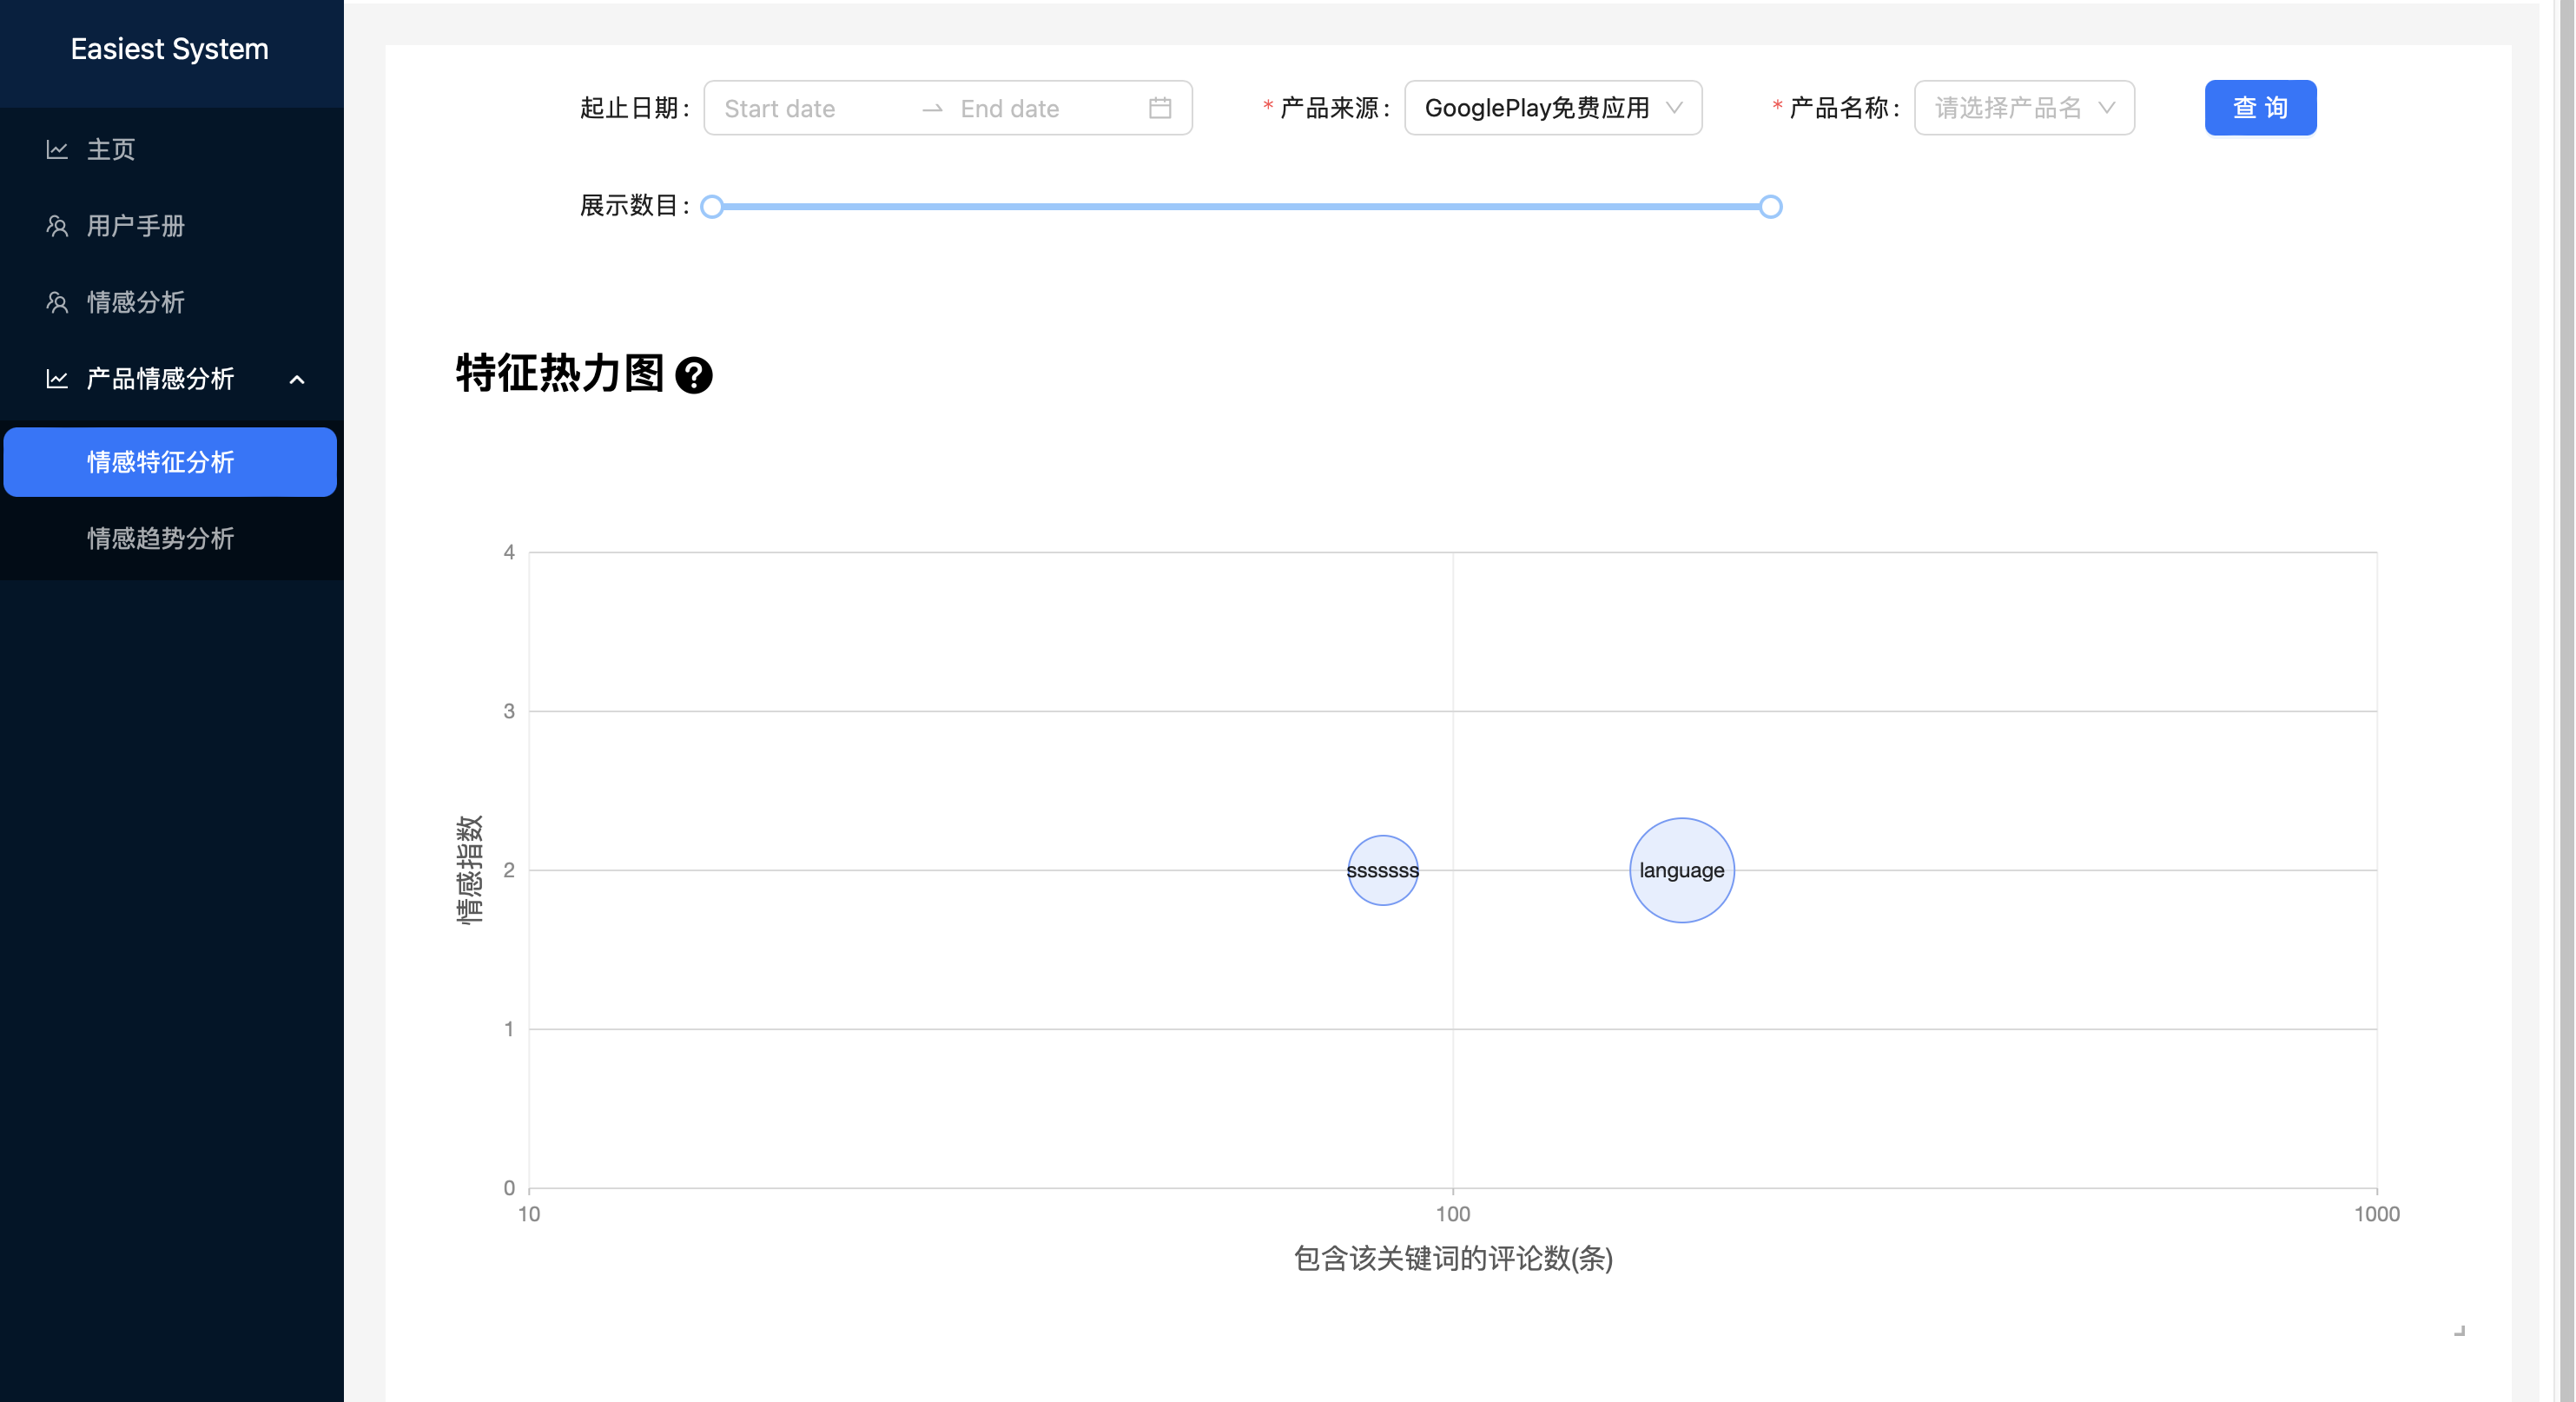
\includegraphics[width=0.98\linewidth]{images/问题5-1.png}
	    \end{minipage}
	}

	\subfloat[特征趋势图初始界面]{
	    \begin{minipage}[t]{0.99\linewidth}
	    \centering
	    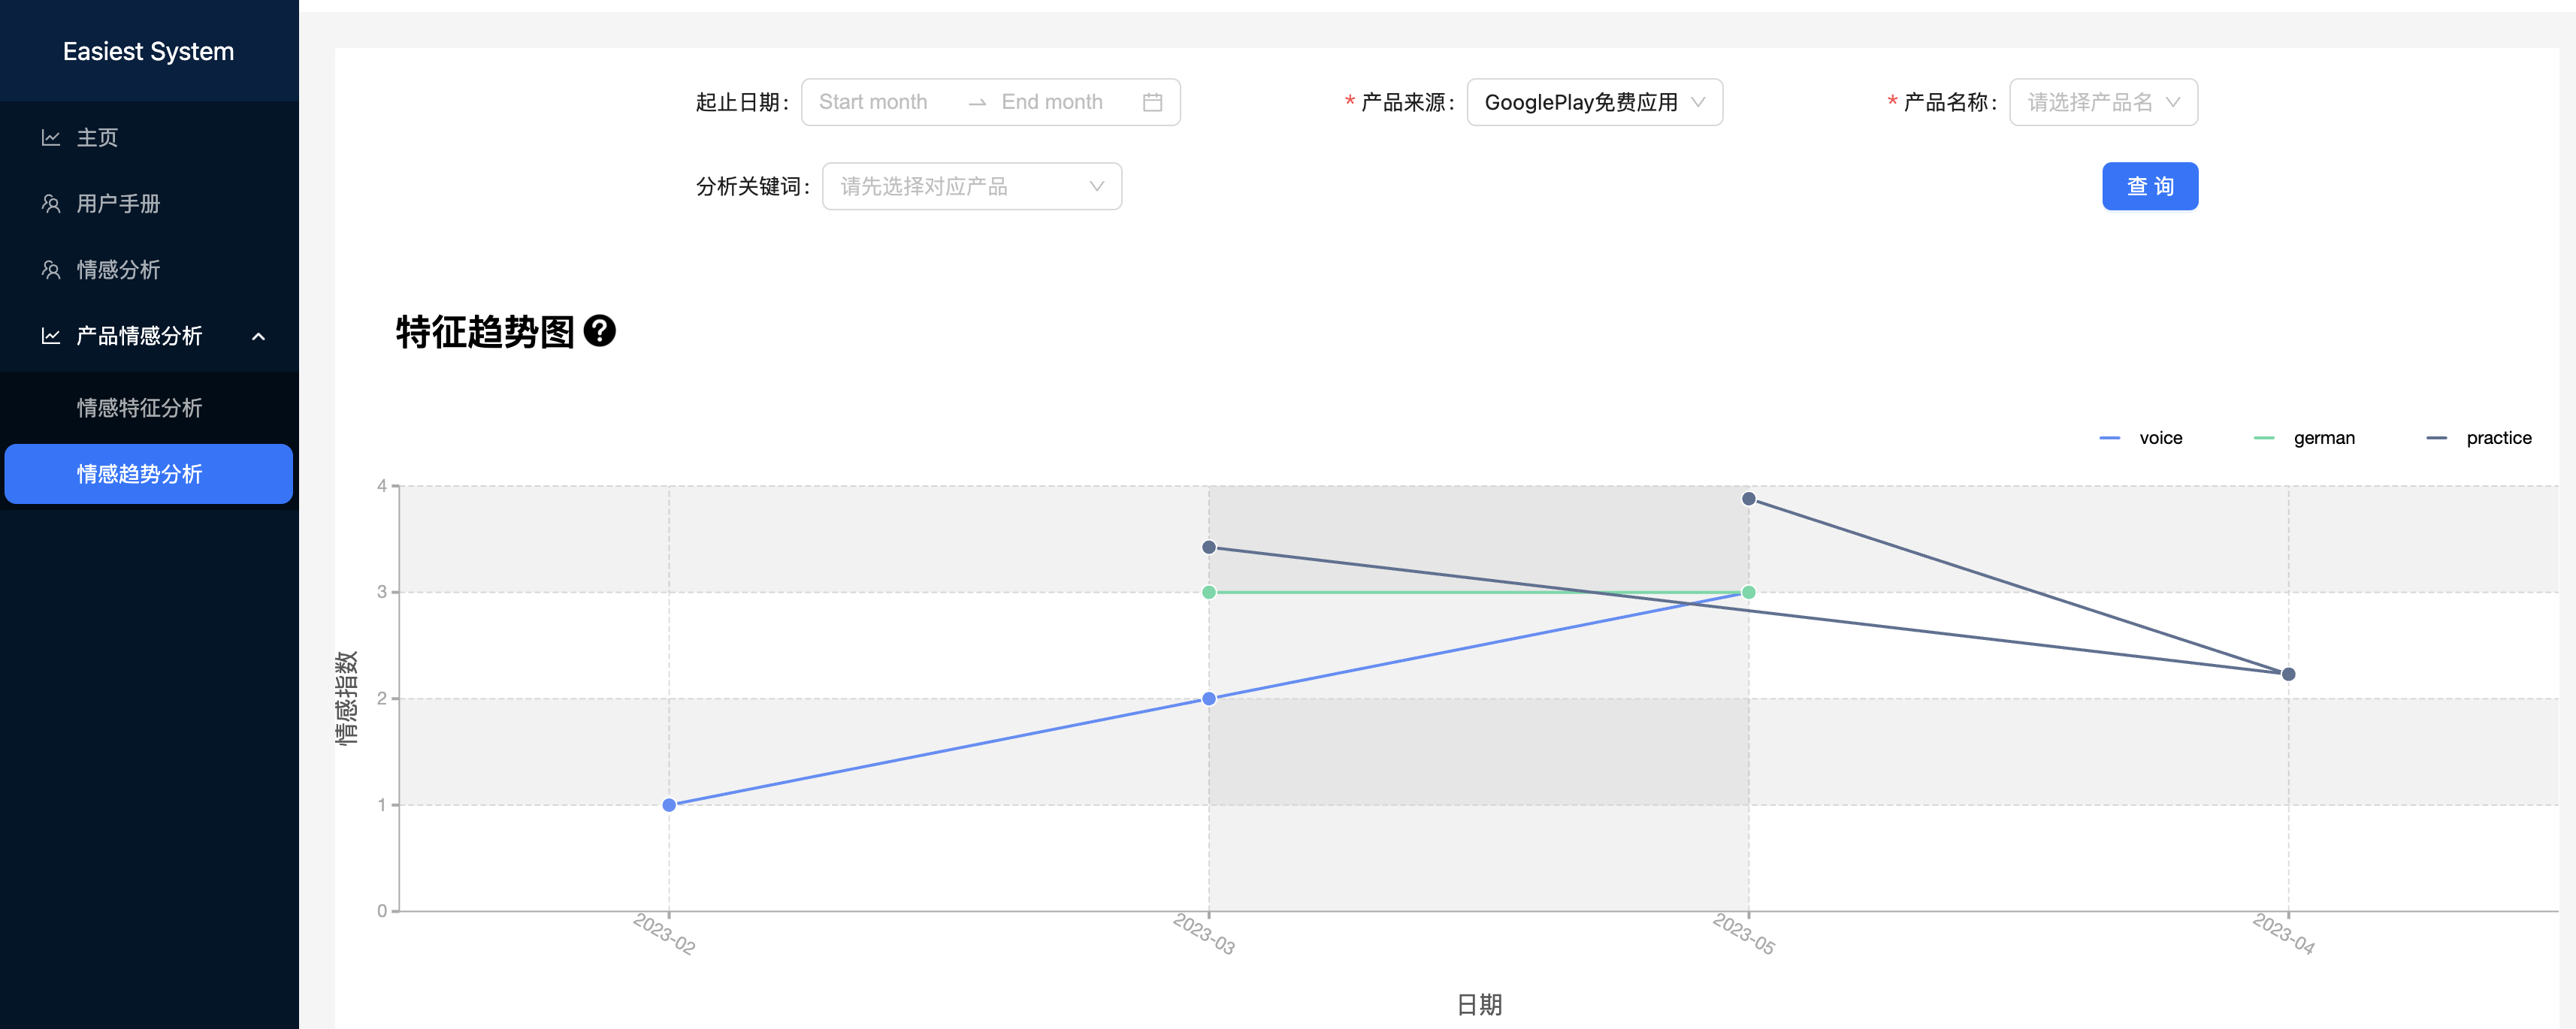
\includegraphics[width=0.98\linewidth]{images/问题5-2.png}
	\end{minipage}
	}
	\centering
	\caption{页面使用无意义的初始值}
    \label{问题5}
\end{figure}

\subsubsection{建议}
这个问题虽然涉及到两个界面,但具体到每个界面的处理还是相对容易的,只需删除初始显示时那些无意义的初值即可,或者在初始显示时对用户进行提示,并换用一些符合现实的初值(而不是这个毫无意义的``sssssss"),让用户理解系统的行为。
